\subsection{TDC Treiber}\label{sec:tdc_driver}

In Code~\ref{code:tdc_driver_header} und \ref{code:tdc_driver_source} ist der selbst entwickelte Firmware-Treiber für
den \acrshort{tdc} dargestellt.

\lstinputlisting[language={c}, label={code:tdc_driver_header}, caption={\acrshort{tdc} Driver (Header)}]{../firmware/Core/TDC/TDC.h}
\lstinputlisting[language={c}, label={code:tdc_driver_source}, caption={\acrshort{tdc} Driver (Source)}]{../firmware/Core/TDC/TDC.c}

\subsection{Python Analyse}\label{sec:python_analyze}

In Code \ref{code:python_analyze} ist das Python-Skript zur Berechnung des arithmetischen Mittelwerts und der
Standardabweichung sowie zum Plotten des Histogramms und des Boxplots dargestellt.

\lstinputlisting[language={python}, label={code:python_analyze}, caption={Python Analyse}]{../utilities/analyze-tof.py}

In Code \ref{code:python_analyze_multi} ist das Python-Skript zur Berechnung des arithmetischen Mittelwerts und der
Standardabweichung sowie zum Plotten der Werte für mehrere Messungen dargestellt.

\lstinputlisting[language={python}, label={code:python_analyze_multi}, caption={Python Analyse (Multi)}]{../utilities/analyze-tofs.py}

\pagebreak

\subsection{Photos}\label{sec:photos}

In Abbildung~\ref{fig:photo_demonstrator_top} und \ref{fig:photo_demonstrator_top_wo_lens} ist der Demonstrator von oben
abgebildet.

\begin{figure}[H]
    \centering
    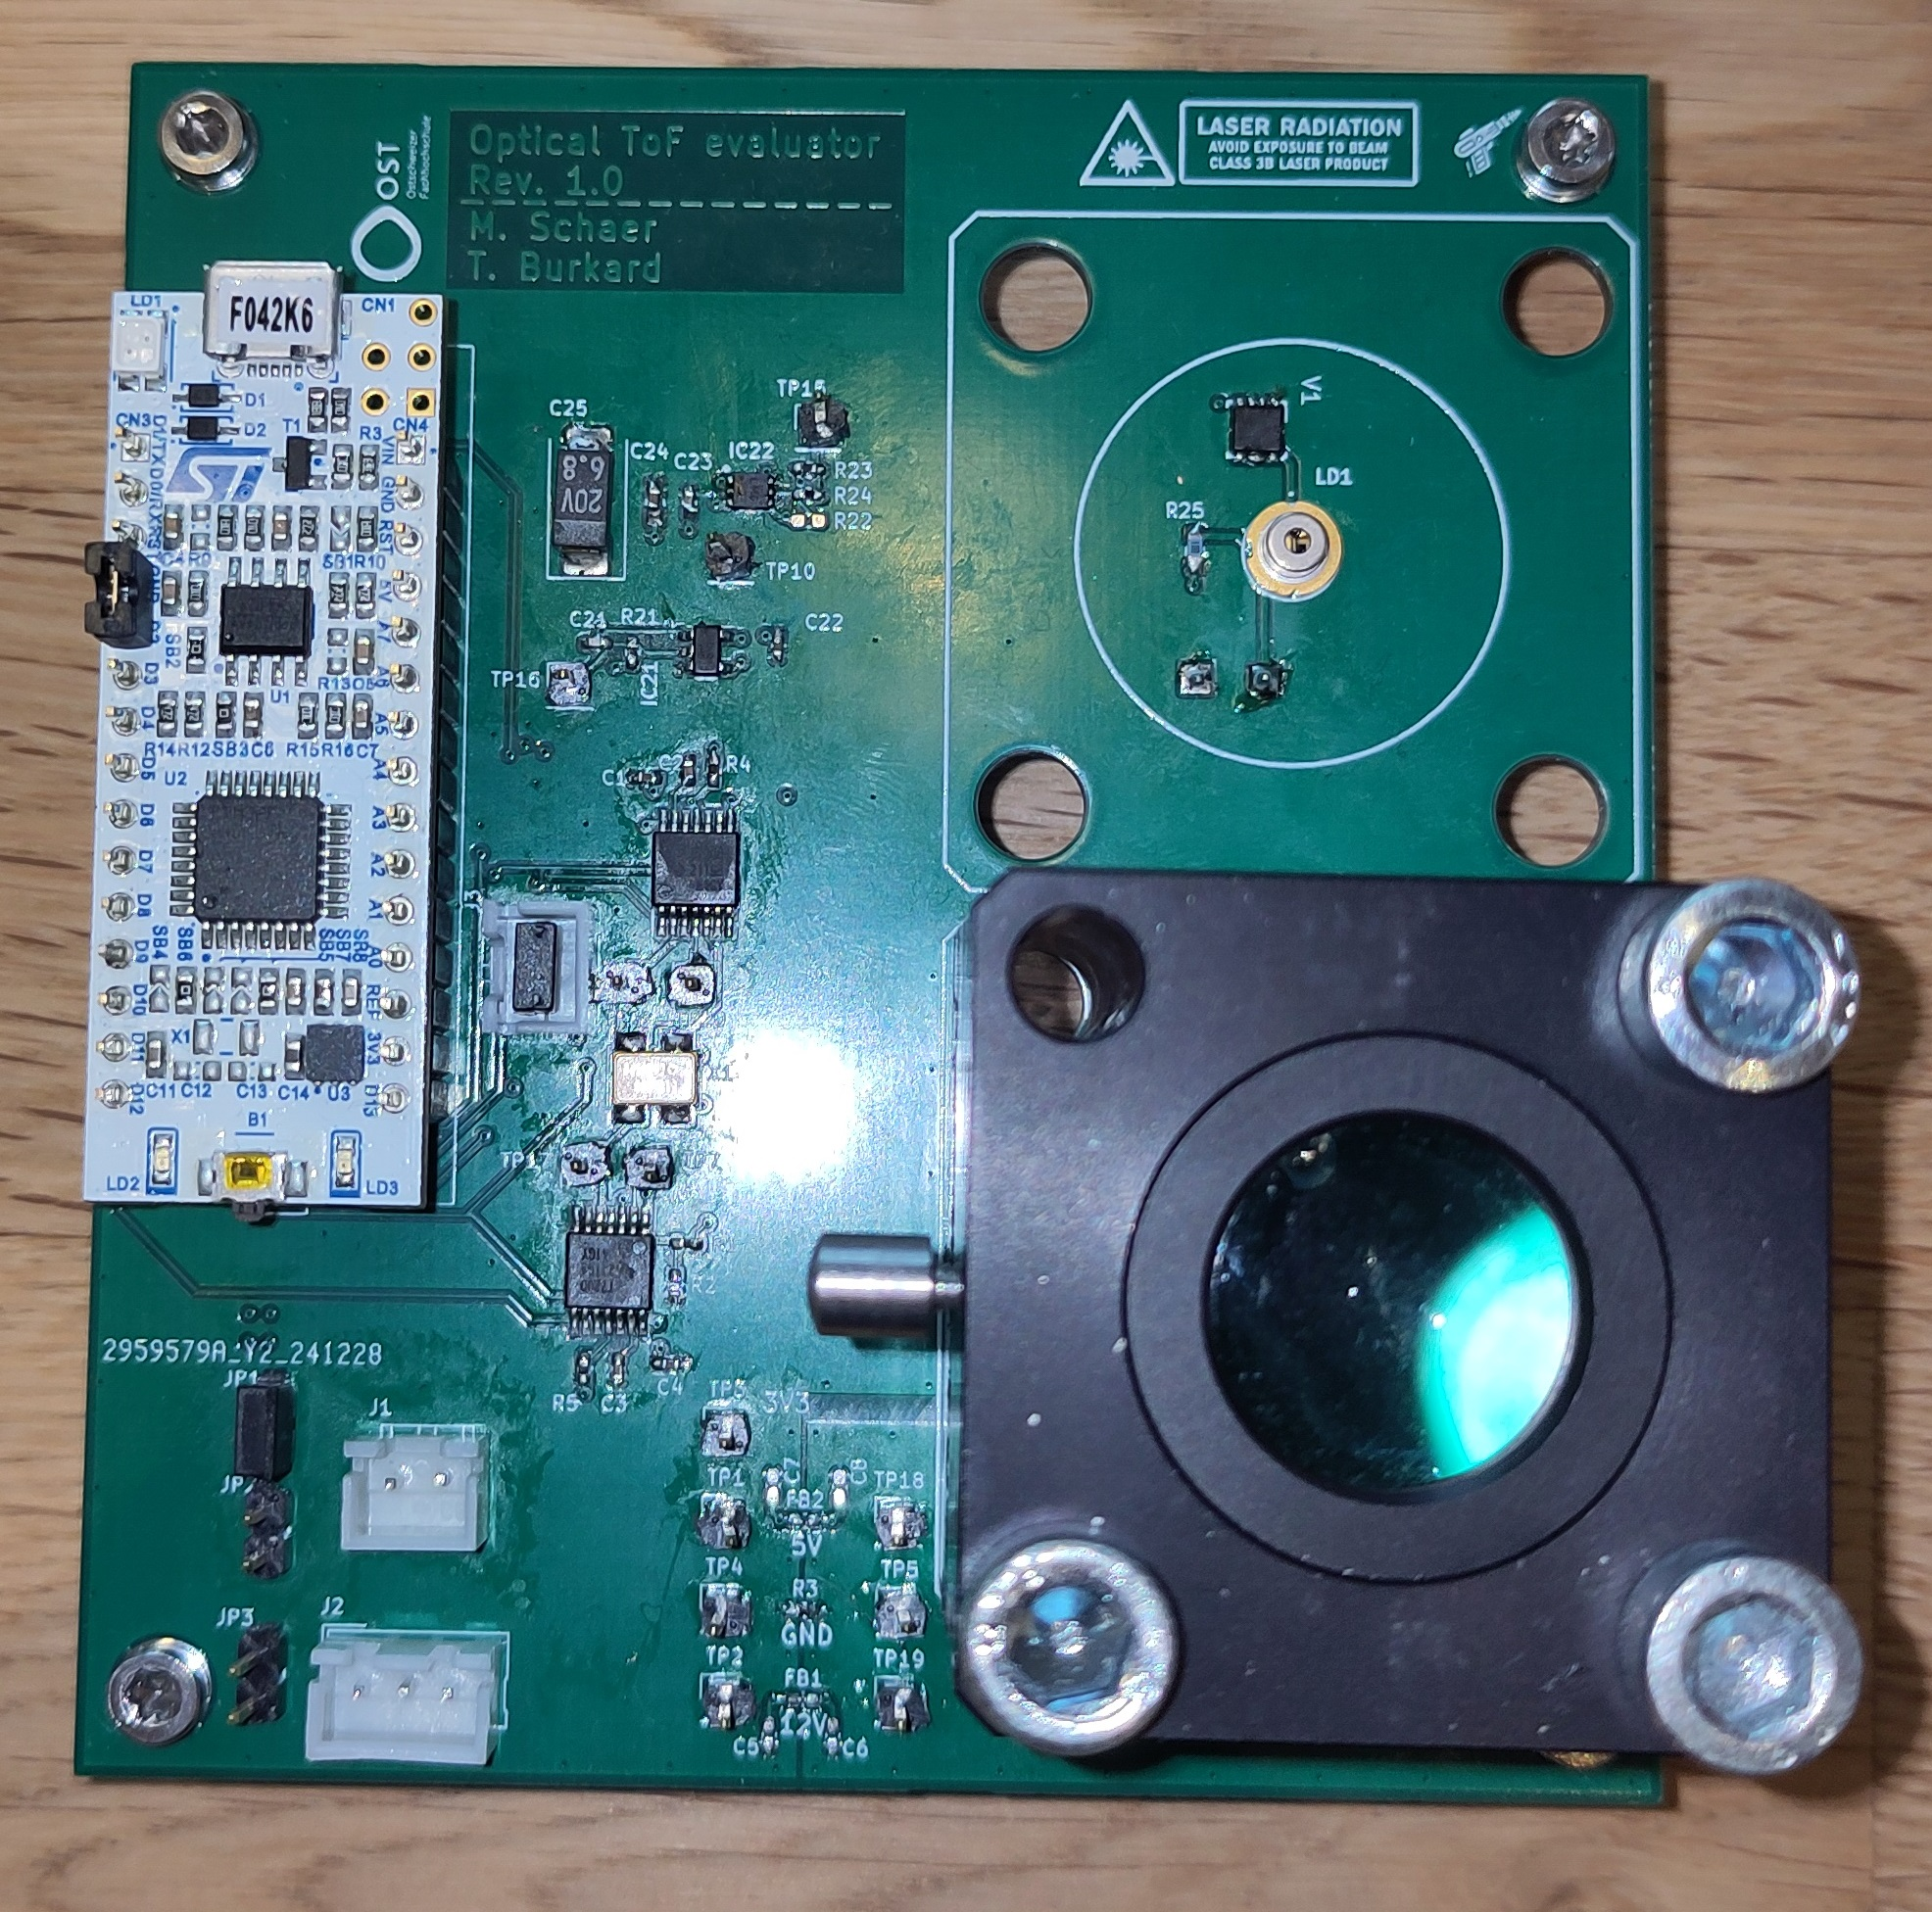
\includegraphics[width=0.6\textwidth]{graphics/photo_demonstrator_top.jpg}
    \caption{Demonstrator von oben}\label{fig:photo_demonstrator_top}
\end{figure}

\begin{figure}[H]
    \centering
    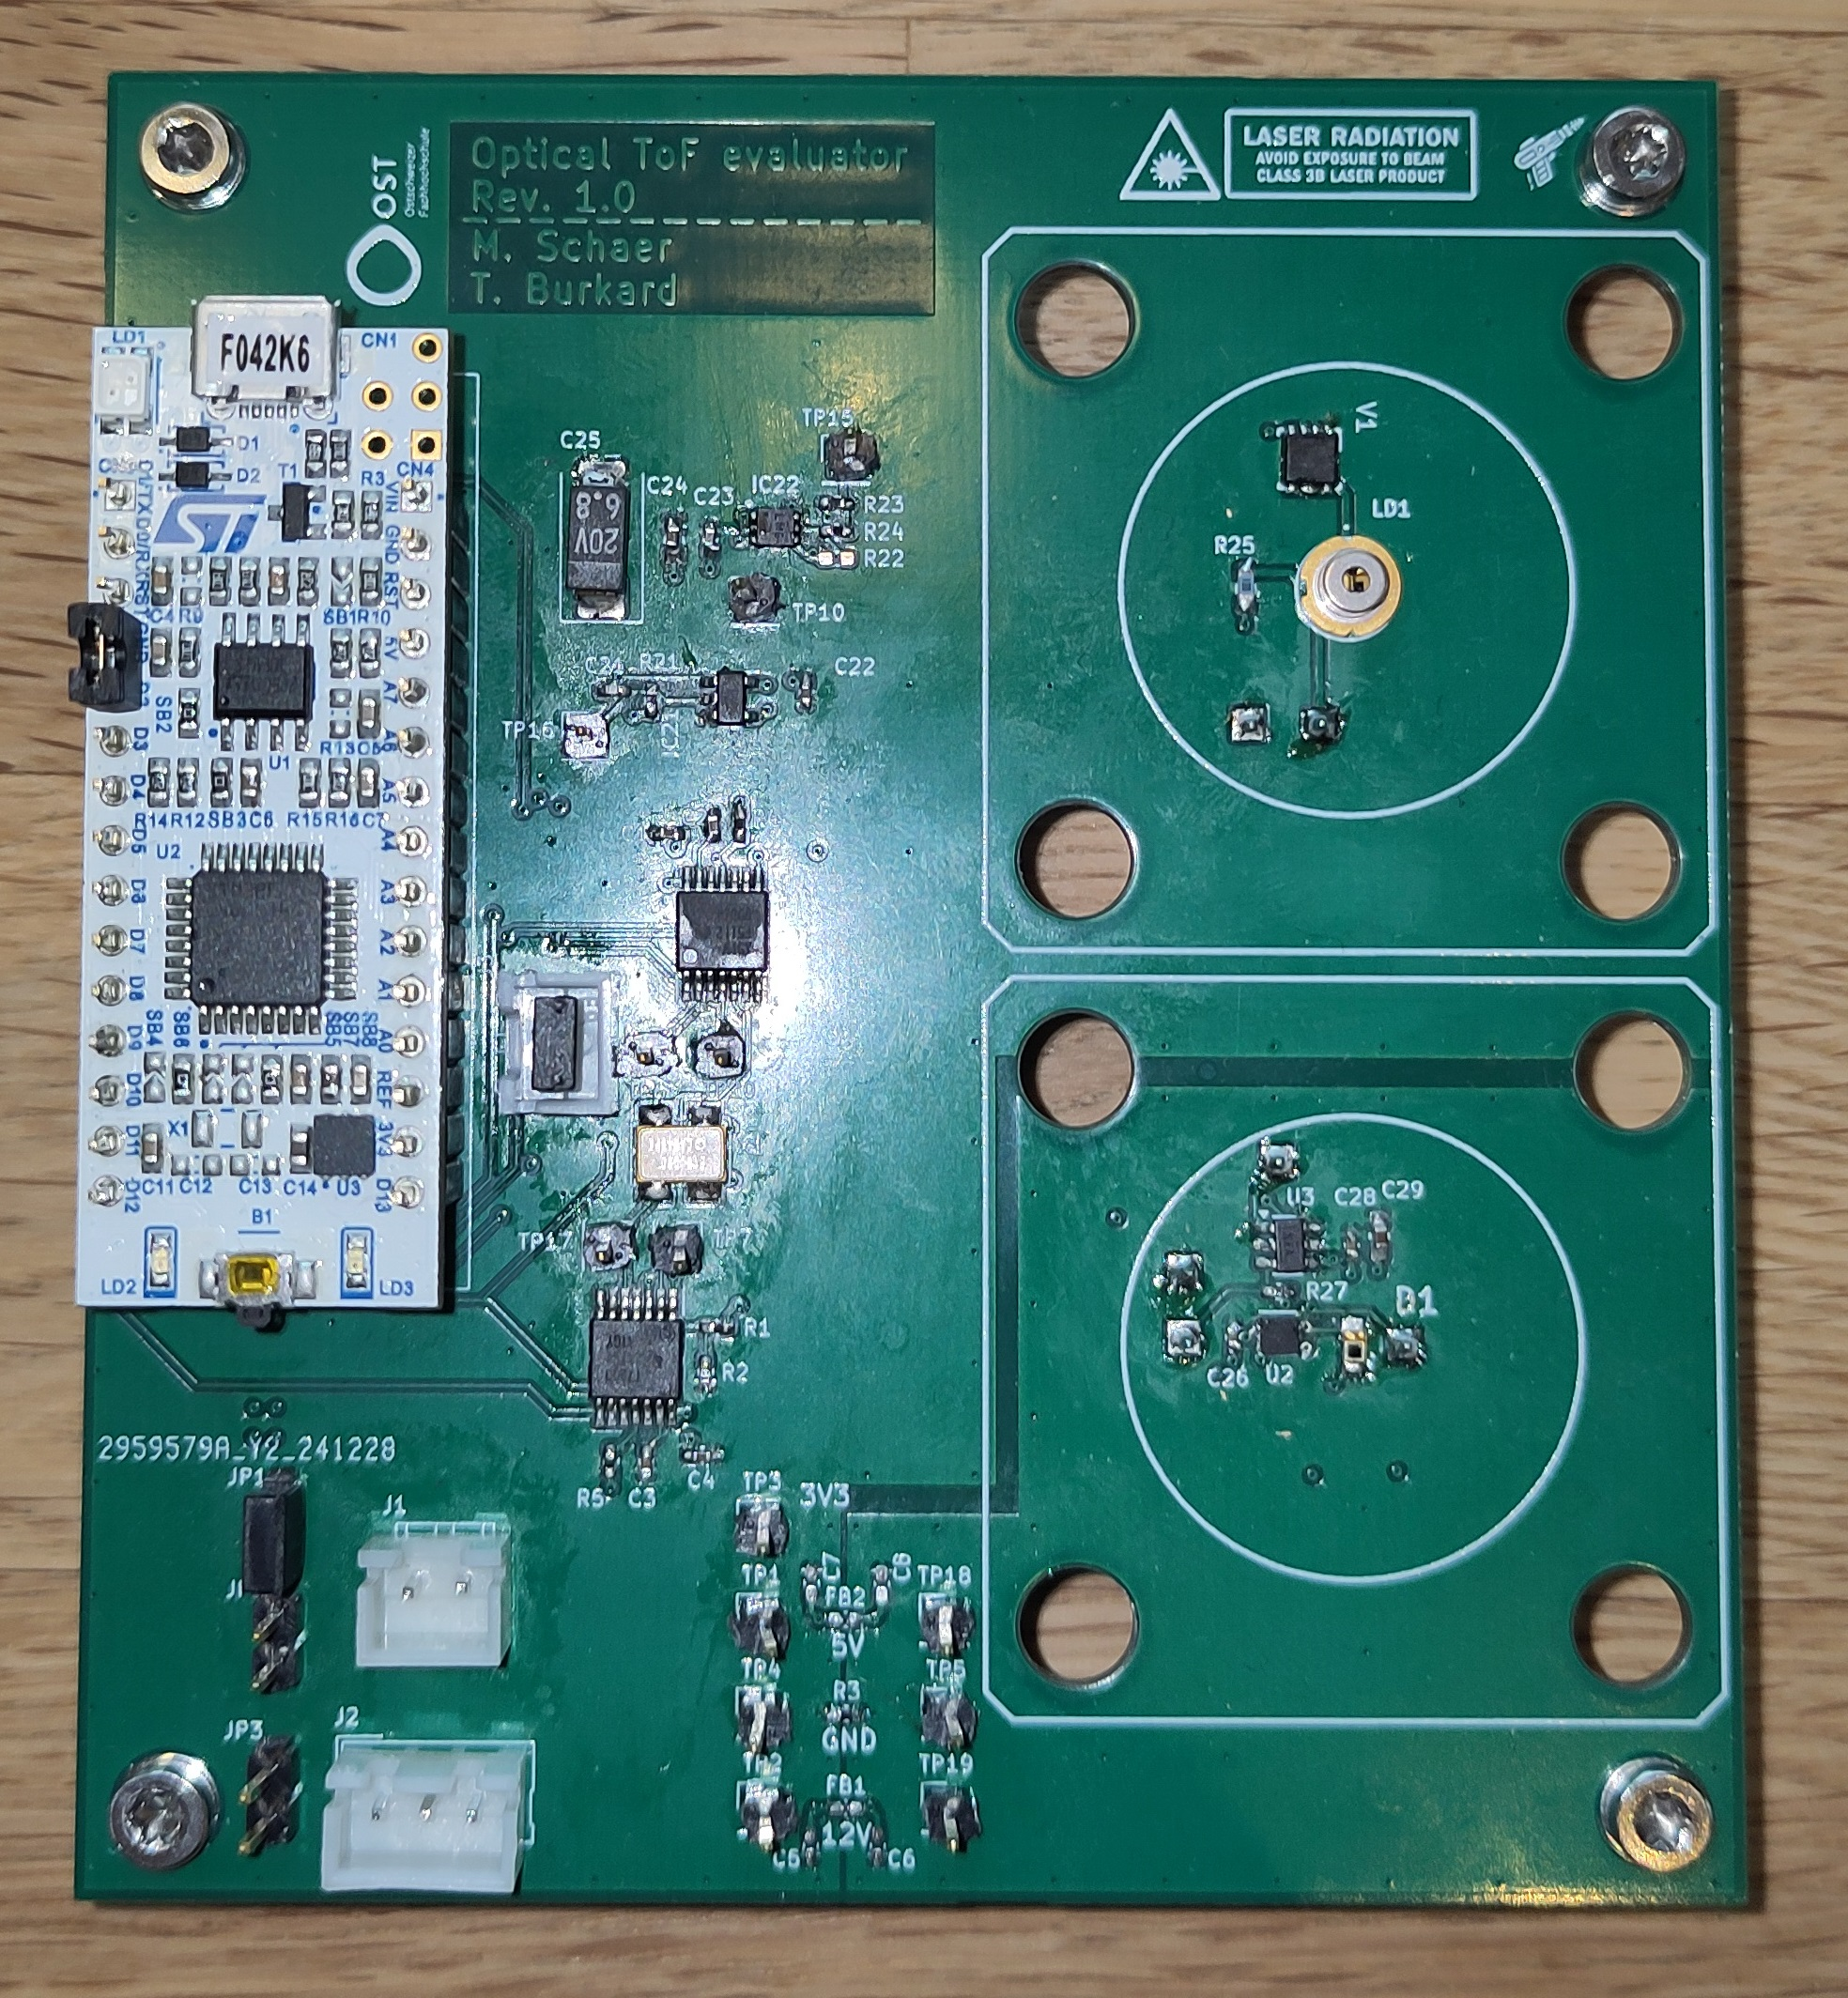
\includegraphics[width=0.6\textwidth]{graphics/photo_demonstrator_top_wo_lens.jpg}
    \caption{Demonstrator von oben ohne Linse}\label{fig:photo_demonstrator_top_wo_lens}
\end{figure}

In Abbildung~\ref{fig:photo_demonstrator_front} und \ref{fig:photo_demonstrator_front_wo_lens} ist der Demonstrator von vorne
abgebildet.

\begin{figure}[H]
    \centering
    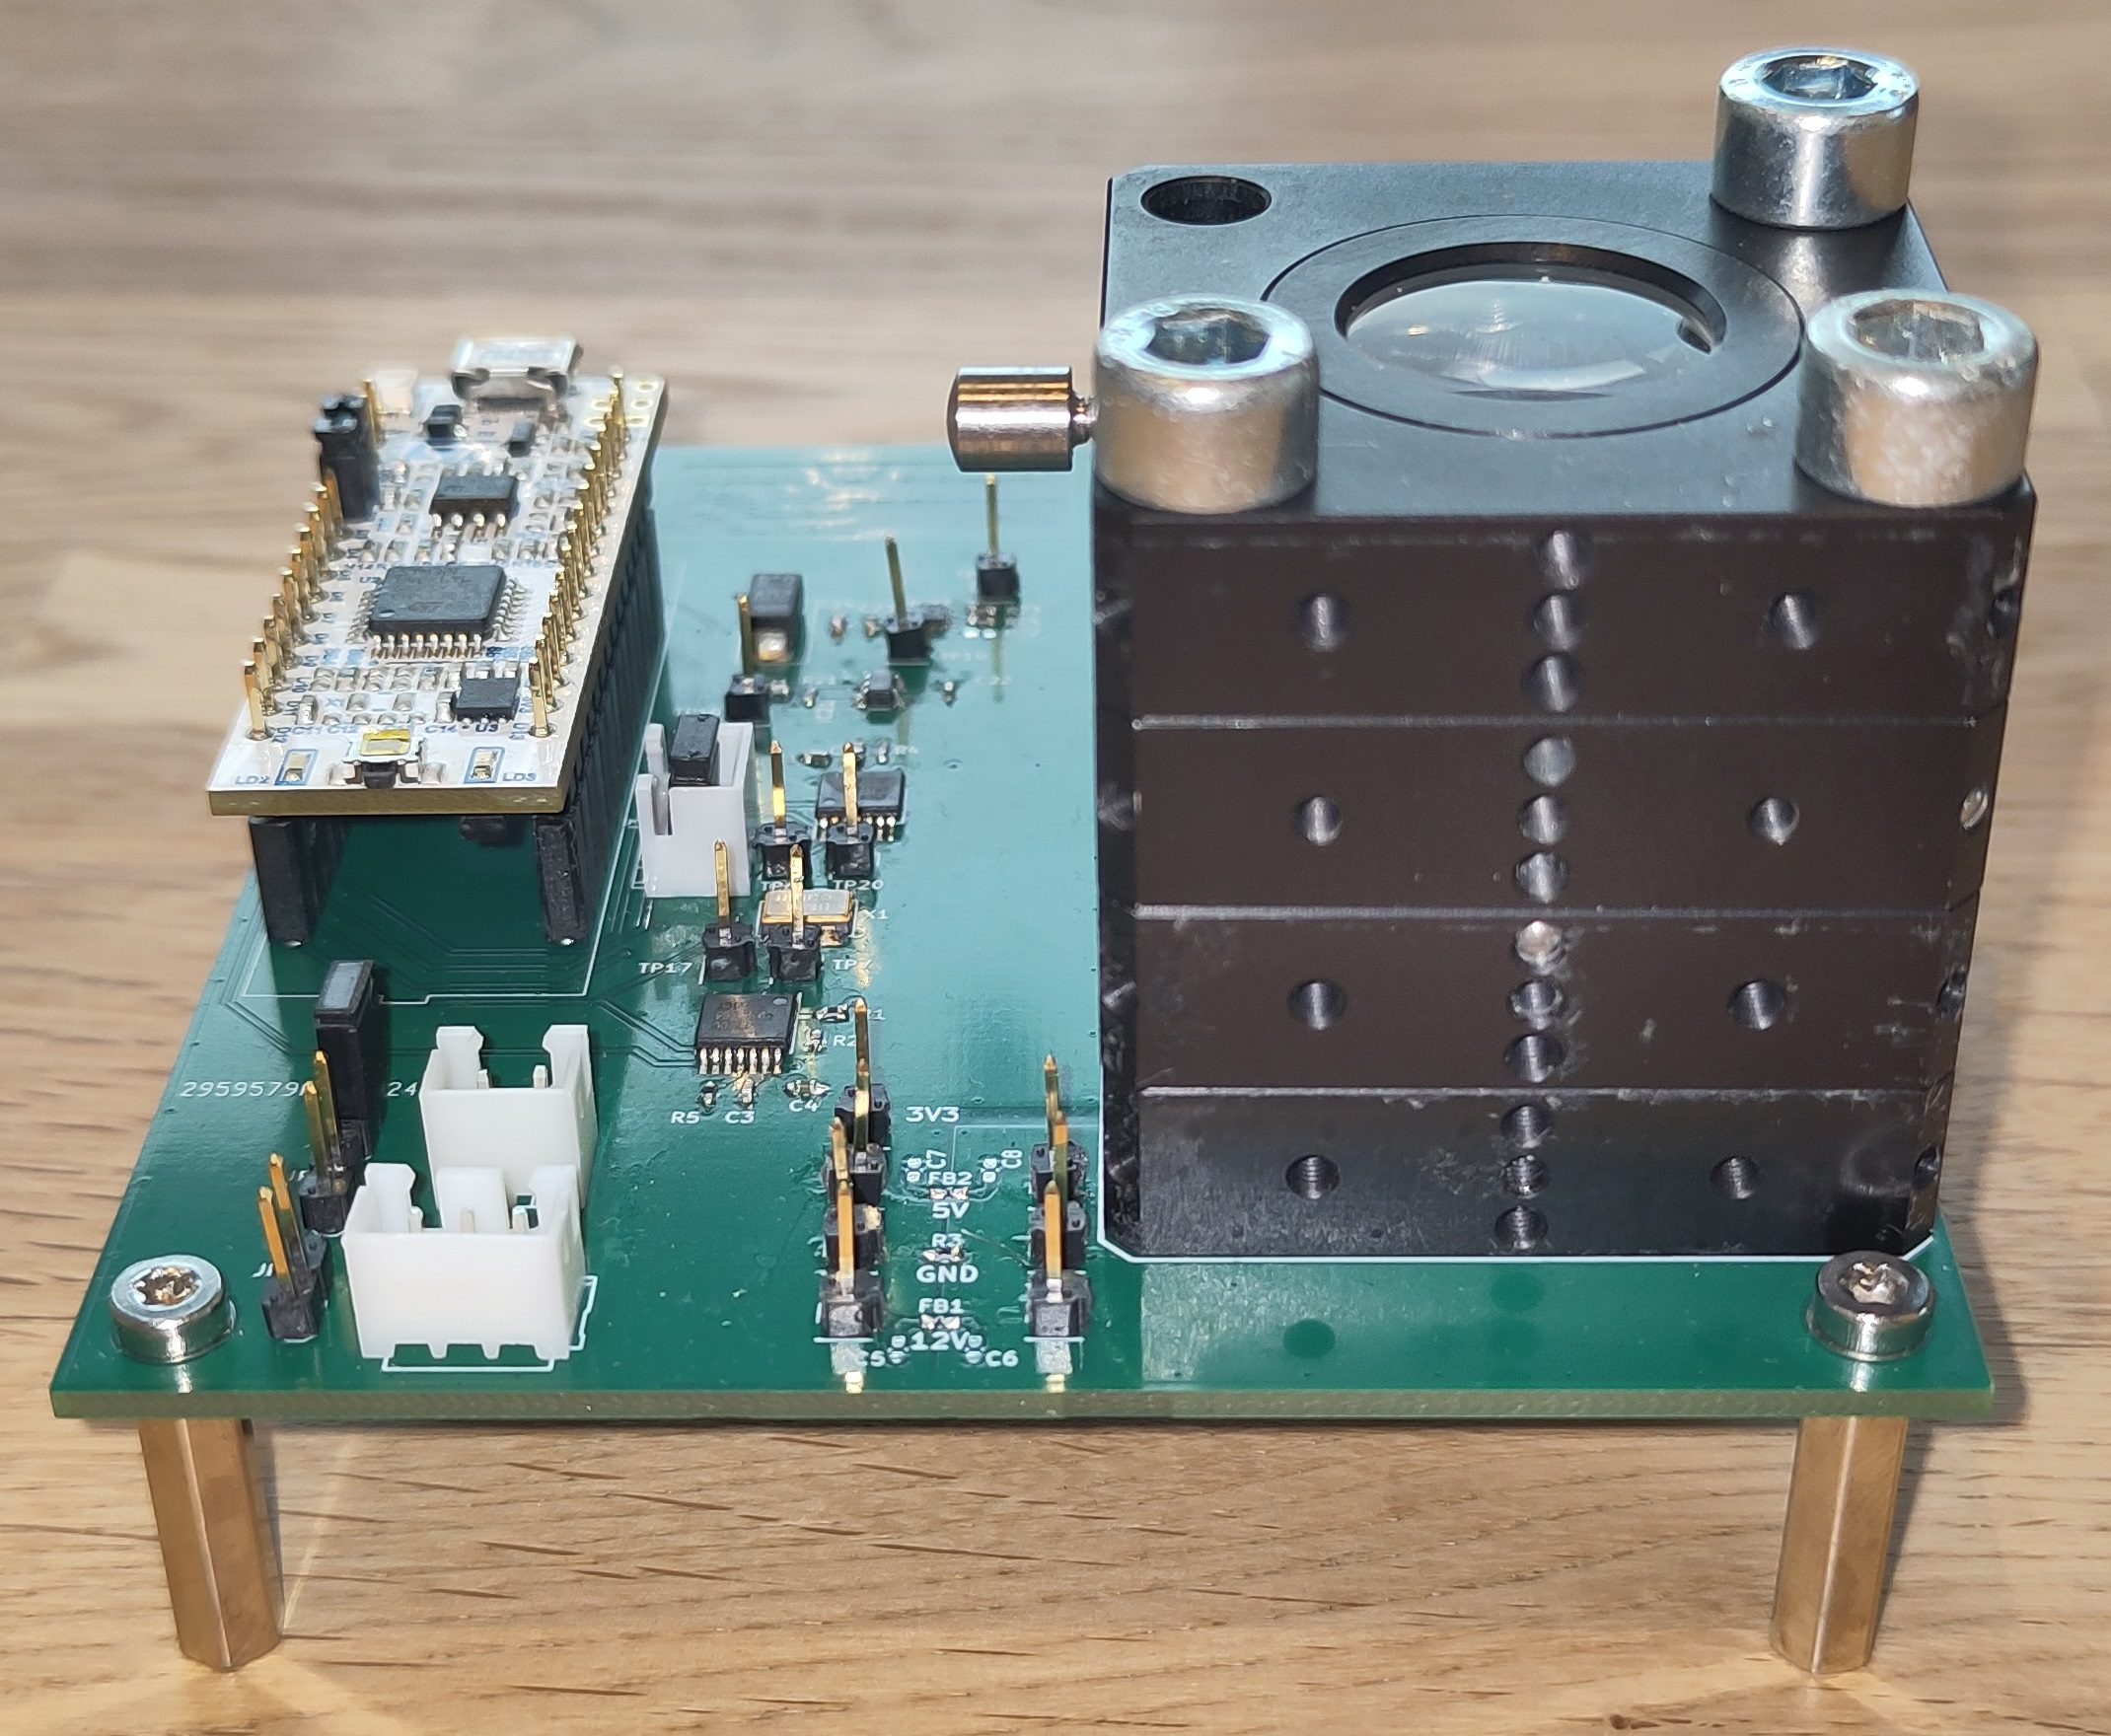
\includegraphics[width=0.6\textwidth]{graphics/photo_demonstrator_front.jpg}
    \caption{Demonstrator von vorne}\label{fig:photo_demonstrator_front}
\end{figure}

\begin{figure}[H]
    \centering
    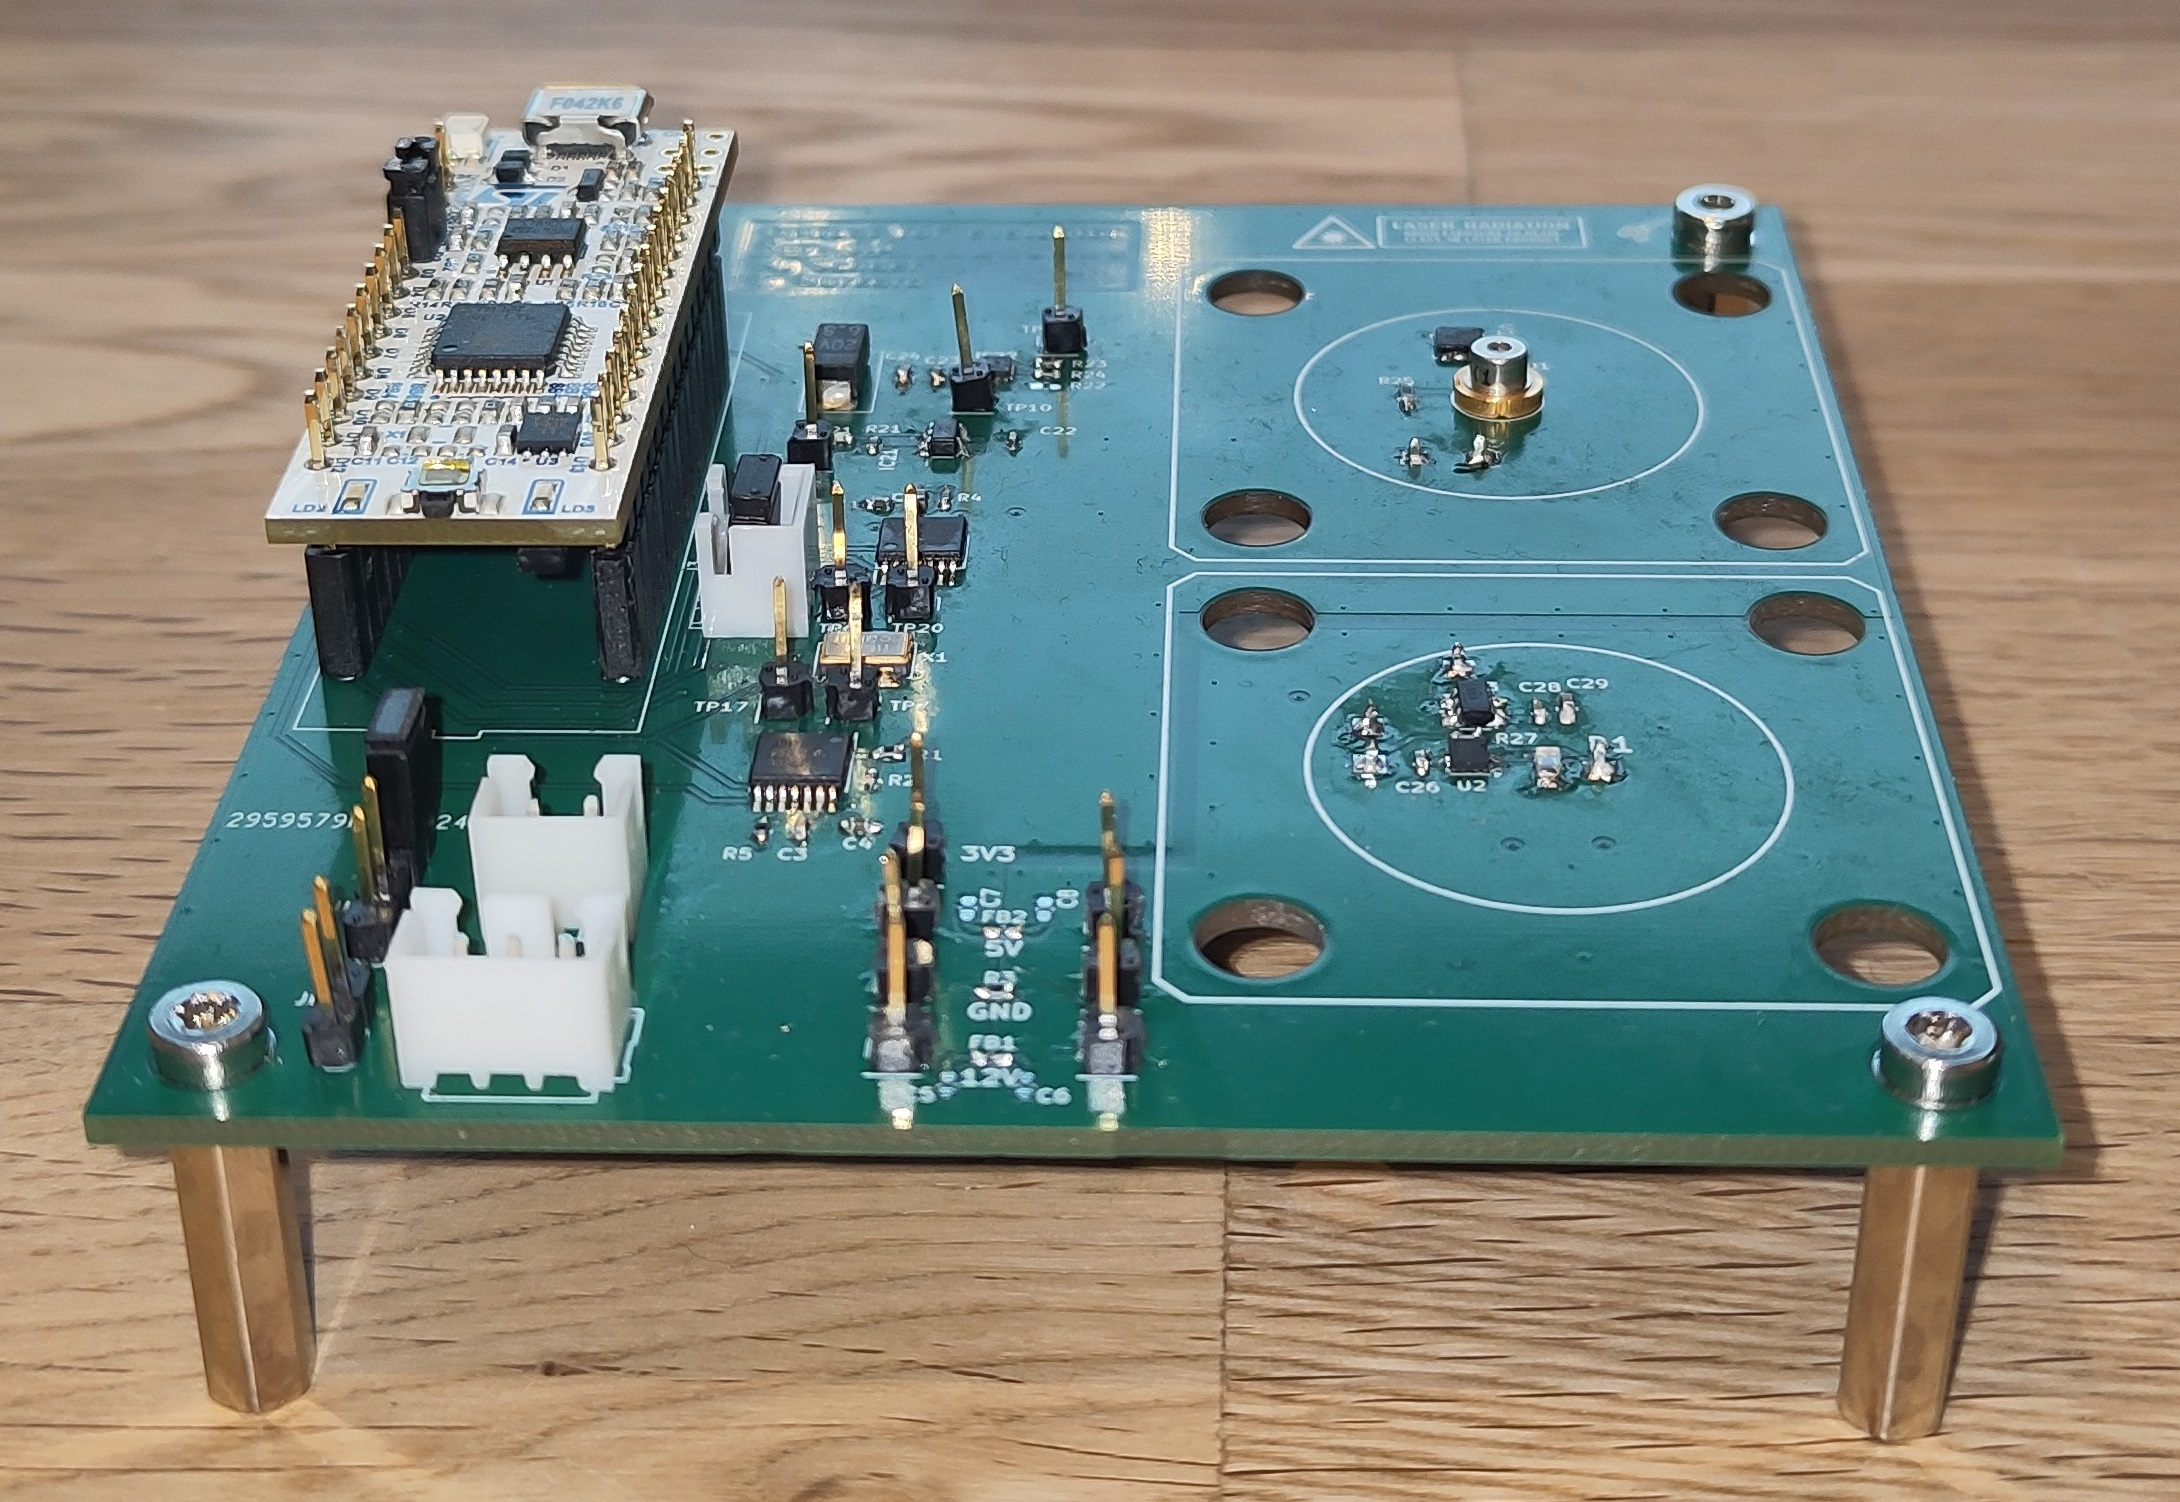
\includegraphics[width=0.6\textwidth]{graphics/photo_demonstrator_front_wo_lens.jpg}
    \caption{Demonstrator von vorne ohne Linse}\label{fig:photo_demonstrator_front_wo_lens}
\end{figure}

In Abbildung~\ref{fig:photo_demonstrator_bottom} ist der Demonstrator von unten abgebildet.

\begin{figure}[H]
    \centering
    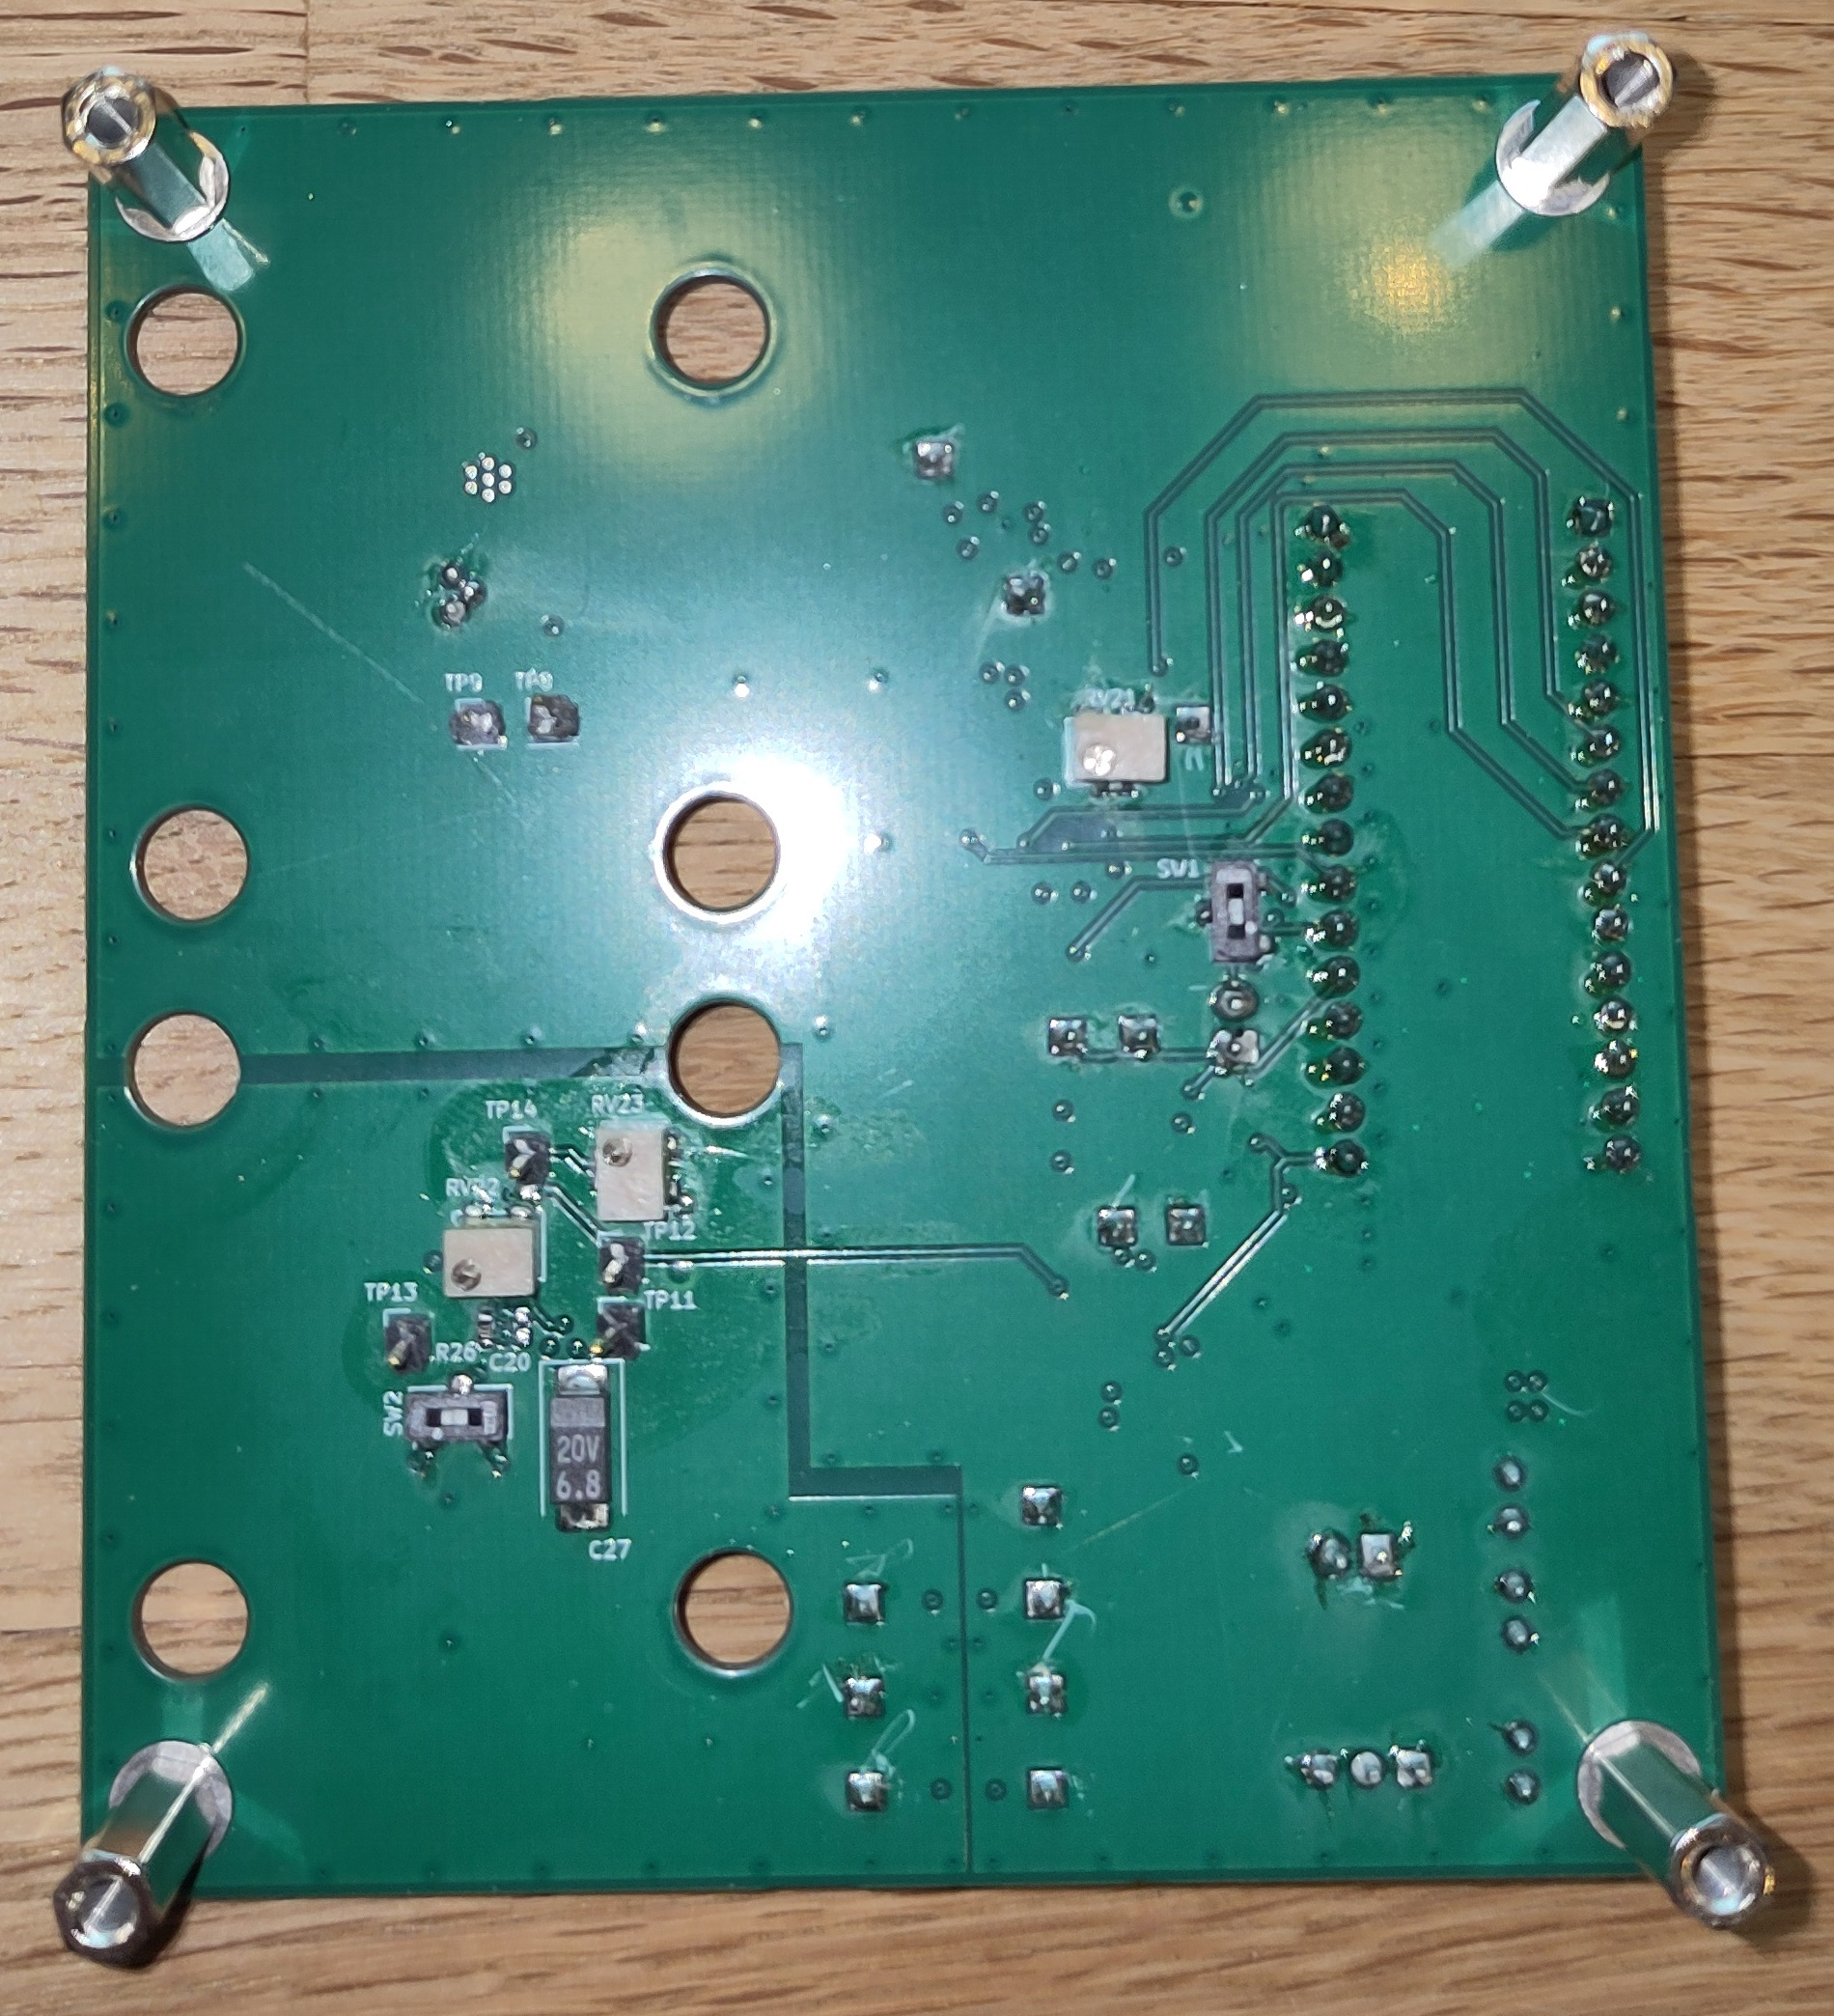
\includegraphics[width=0.6\textwidth]{graphics/photo_demonstrator_bottom.jpg}
    \caption{Demonstrator von unten}\label{fig:photo_demonstrator_bottom}
\end{figure}

\begin{landscape}

    \subsection{Schema}\label{sec:schematic_apdx}
    \global\pdfpageattr\expandafter{\the\pdfpageattr/Rotate 90}
    \begin{figure}[H]
        \centering
        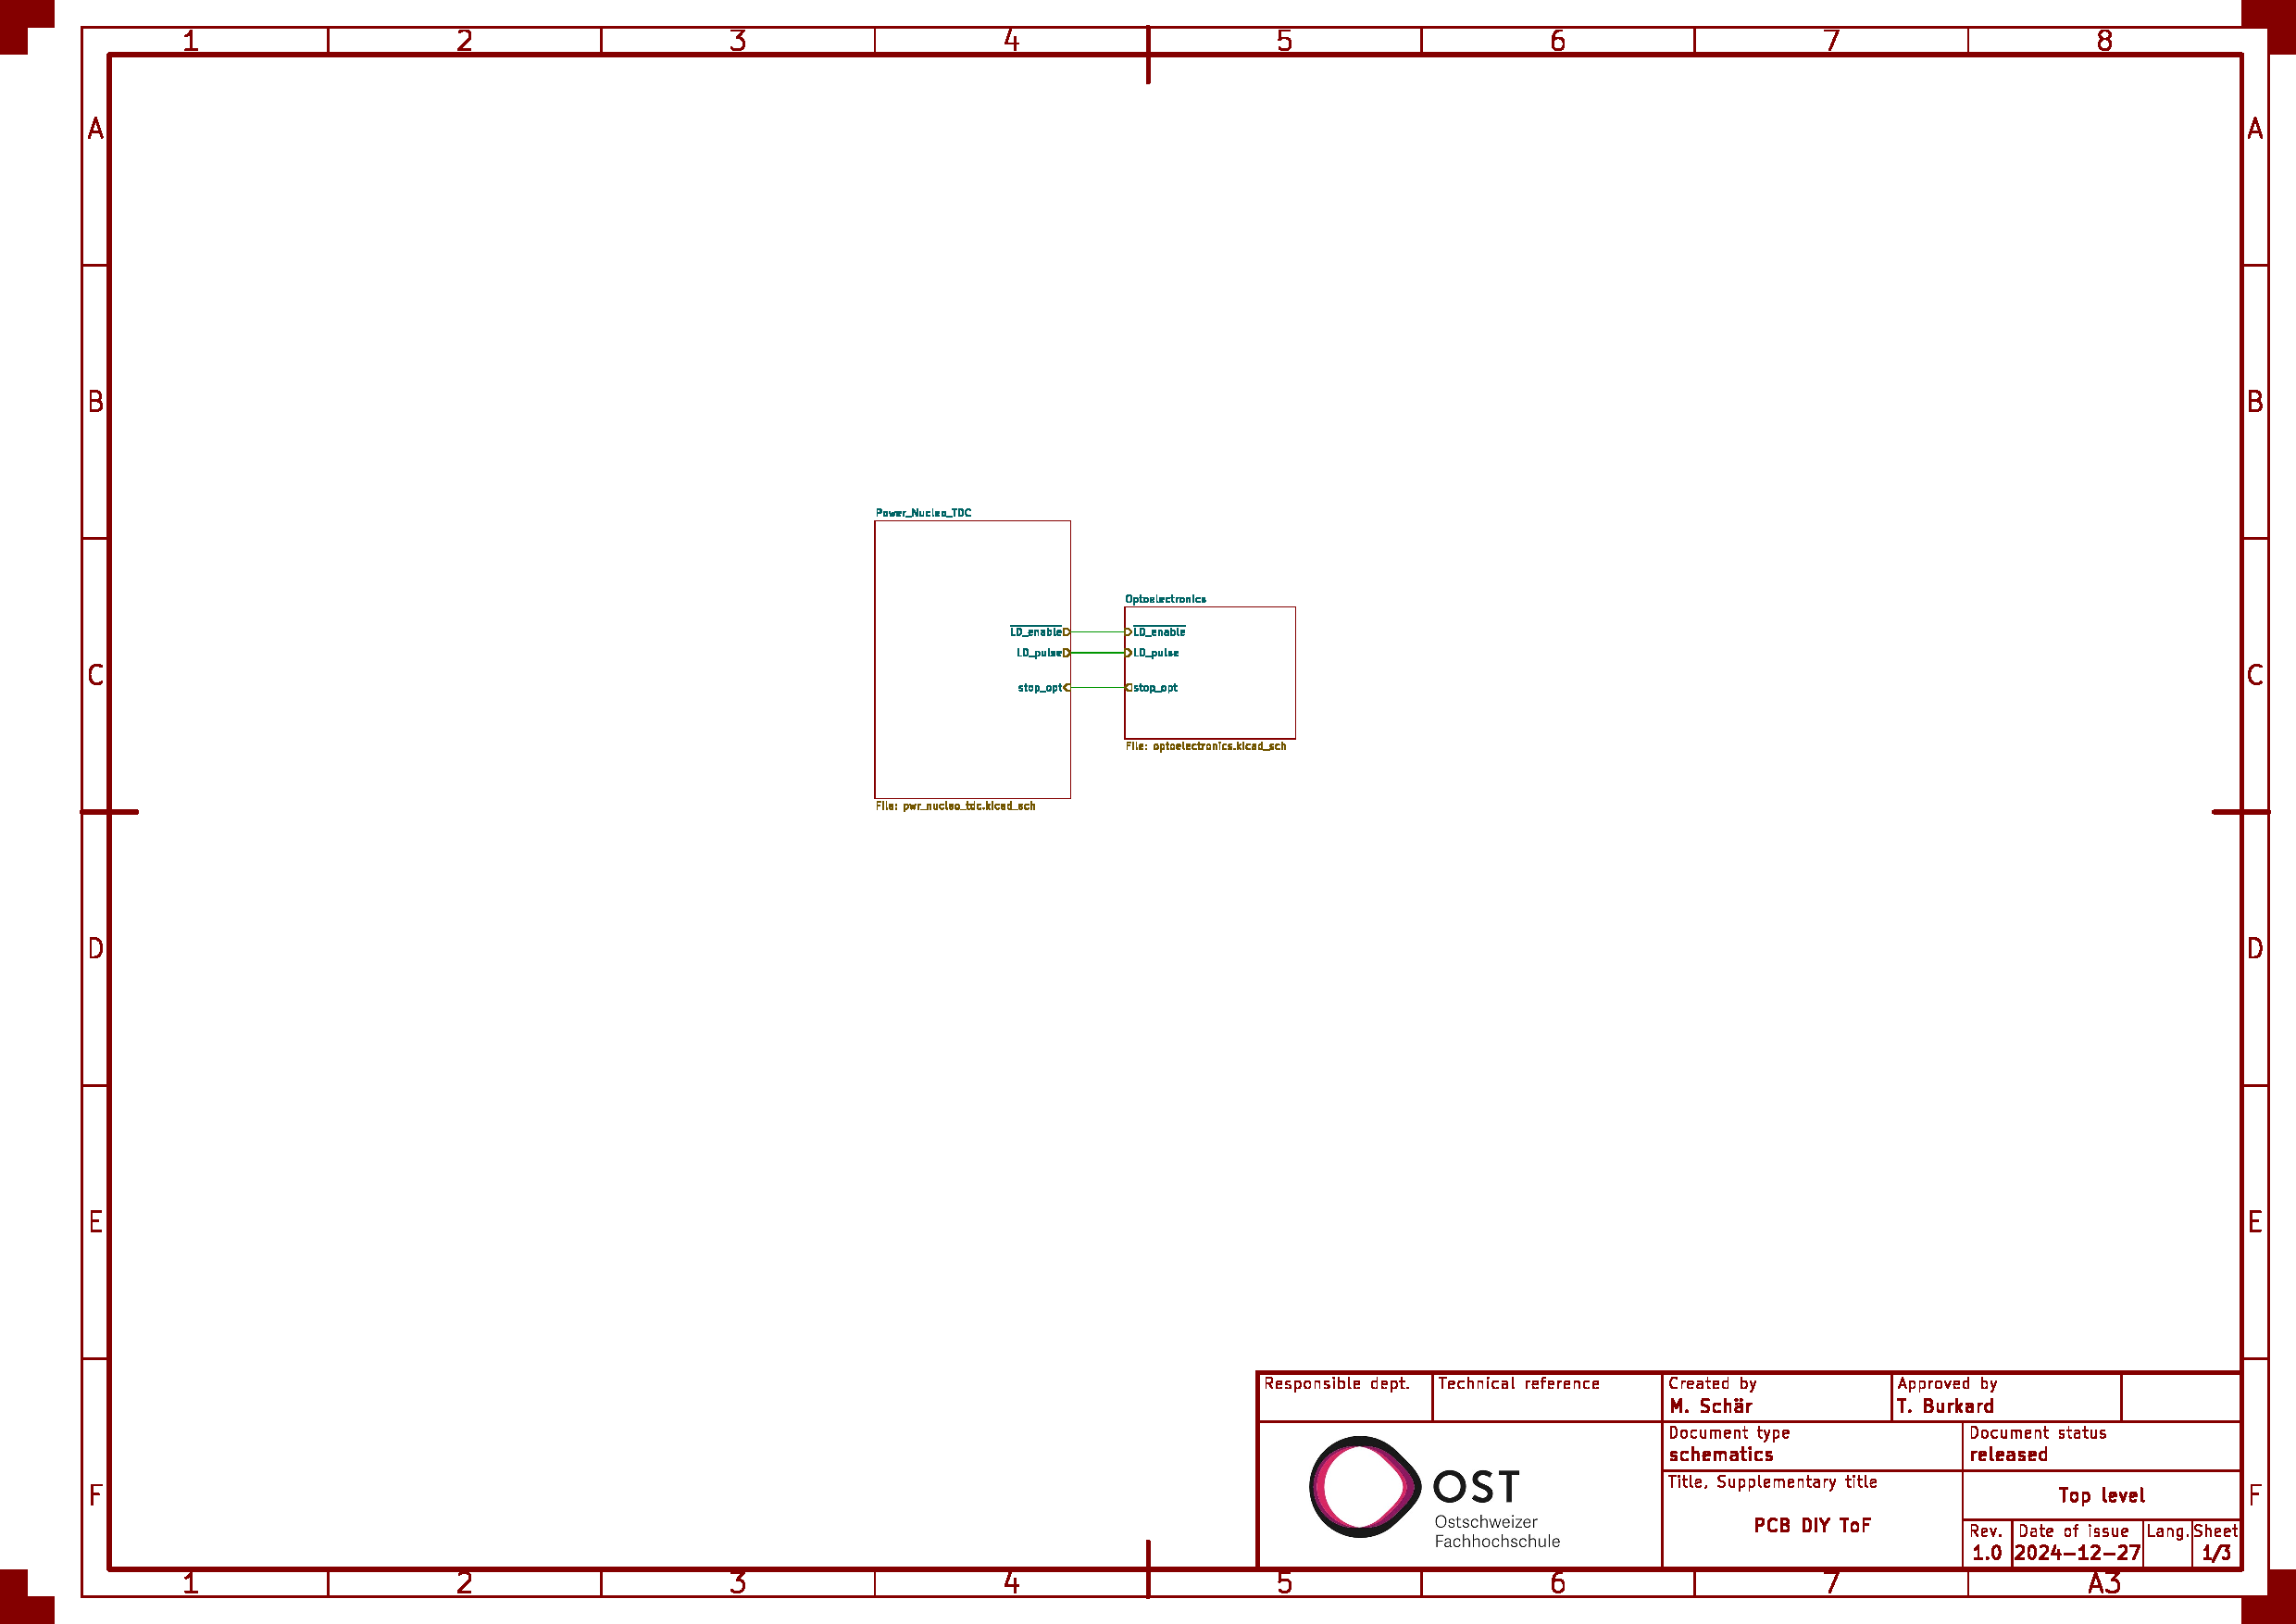
\includegraphics[page=1, width=1.2\textwidth]{attachments/schematic.pdf}
        \caption{Schema S.1/3}\label{fig:schematics_1}
    \end{figure}
    \pagebreak

    \global\pdfpageattr\expandafter{\the\pdfpageattr/Rotate 90}
    \begin{figure}[H]
        \centering
        \includegraphics[page=2, width=1.2\textwidth]{attachments/schematic.pdf}
        \caption{Schema S.2/3}\label{fig:schematics_2}
    \end{figure}
    \pagebreak

    \global\pdfpageattr\expandafter{\the\pdfpageattr/Rotate 90}
    \begin{figure}[H]
        \centering
        \includegraphics[page=3, width=1.2\textwidth]{attachments/schematic.pdf}
        \caption{Schema S.3/3}\label{fig:schematics_3}
    \end{figure}
    \pagebreak


    \subsection{Stückliste}

    \begin{table}[H]
        \scriptsize
        \mytable
            {|l|l|l|l|l|l|}
            {\textbf{Reference} & \textbf{Value} & \textbf{Datasheet} & \textbf{Footprint} & \textbf{Qty} & \textbf{DNP}}
            {\Reference & \Value & \Datasheet & \Footprint & \Qty & \DNP}
            {tables/bom.csv}
        \caption{Bill of Material}\label{tab:bom}
    \end{table}

\end{landscape}

\global\pdfpageattr\expandafter{\the\pdfpageattr/Rotate 0}
